\scanpage{37}
\mspage{18}
\uline{Complément}. Retour sur une démonstration \uline{géométrique} du th. 2, cor. 1 b). OPS que $G$ est \unsure{la} jacobienne généralisée de $Y$, et il suffit de montrer le

\uline{Lemme} Soit $Y$ une variété élémentaire d'Artin anabélienne, (sur $K$ alg. clos), $Y\hookrightarrow J_Y^1$ son plongement dans sa jacobienne généralisée, $u\in J_Y^0(k)$ et $U$ un ouvert non vide de $Y$, tels que $U+u\subset Y$. Alors $u=1$\inserted{, ou encore : l'application \unsure{$x\mapsto xu$|$x\mapsto x+u$} de $U$ dans $Y$ est l'identité.}
\figure{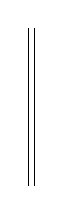
\begin{tikzpicture}\draw (0,0)--(0,2);\draw (.08,0)--(.08,2);\end{tikzpicture}}

Par dévissage, on est ramené au cas où $Y$ est une courbe. Supposons la d'abord complète, de sorte que $U+u\subset Y$ implique $Y+u\subset Y$ -- alors le résultat est bien connu. \unsure{Cela|Cet} résulte p.ex. de la formule des pts fixes, qui implique que $\tau_u|_Y$ \inserted{si ce n'est l'identité,} a $2-2g$ pts fixes, ce qui (comme $g\geq2$ à cause de l'hypothèse anabélienne) est absurde.

Cela \deleted{signifie} \inserted{implique} donc, dans le cas général, \inserted{au moins si $g\neq1$,} que l'image de $u$ dans la partie abélienne de $J_Y^0(k)$ est nulle.

\margin{Si $g\geq2$, quitte à remplacer $Y$ par $\widehat Y$, OPS. $Y$ complète. Si $g=1$ ou 0, cf argument homologique plus bas}
\margin{\unsure{ne sert à rien ici}}

\deleted{[Or d'après la structure connue de $J_Y^0$ comme extension de $J_{\widehat Y}^0$ par un tore $\mathbb G_m^I/\mathbb G_m$ (où $I=\widehat Y-Y$) $u$ s'identifie à un élément de $(\mathbb G_m^I/\mathbb G_m)(k)$, donc est défini par $(\lambda_i)_{i\in I}$, les $\lambda_i\in k^*$, qui servent à construire un fibré inversible}
\margin{36}
